\subsection*{Фигуры из презентации в файл MS Excel}
\addcontentsline{toc}{subsection}{Фигуры из презентации в файл MS Excel}

\textbf{Задание:}\\
Поместить в область просмотра несколько фигур из палитры Презентация. Запишите в файл Excel данные о размещённых фигурах -- тип фигуры и параметры.\\

\textbf{Решение:}\\
Для того, чтобы связать Excel файл с моделью, необходимо использовать блок -- файл Excel. Далее были расставлены элементы презентации. Для выгрузки была создана кнопка \textit{Save}. (Рисунок \ref{fig:excel3})
\begin{figure}[h]
	\centering 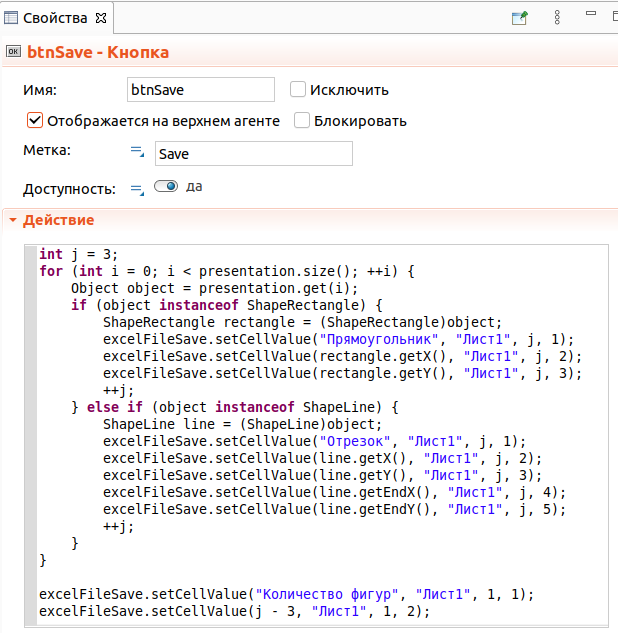
\includegraphics[scale=0.4]{excel3}
	\caption{Логика кнопки для выгрузки данных из файла}
	\label{fig:excel3}
\end{figure}

\newpage

При нажатии на данную кнопку происходит сохранение фигур заданных типов с заданными параметрами. (Рисунок \ref{fig:excel4})
\begin{figure}[h]
	\centering 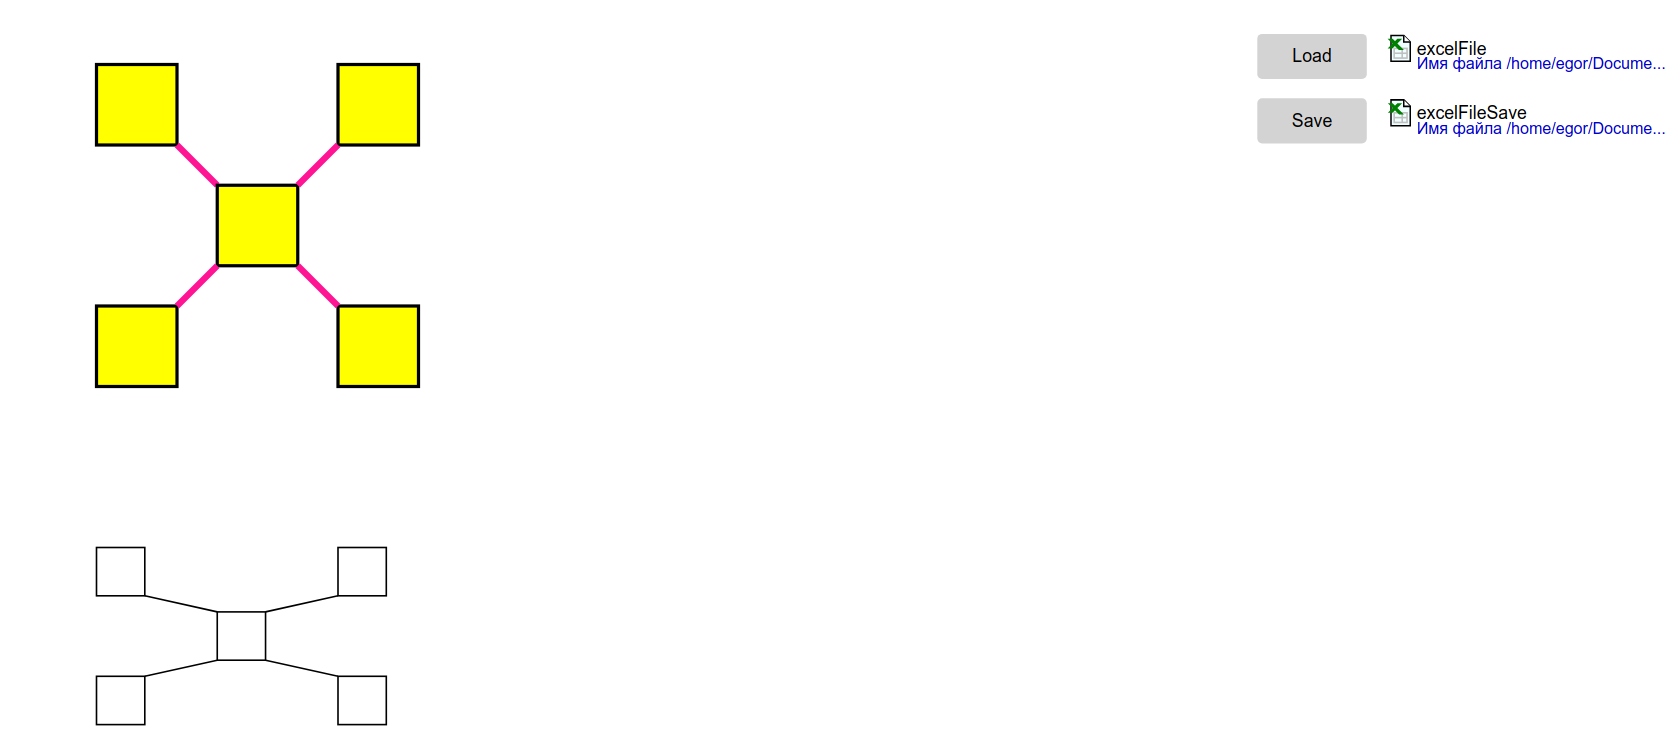
\includegraphics[scale=0.25]{excel4}
	\caption{Результат нажатия на кнопку \textit{Save}}
	\label{fig:excel4}
\end{figure}

\begin{figure}[h]
	\centering 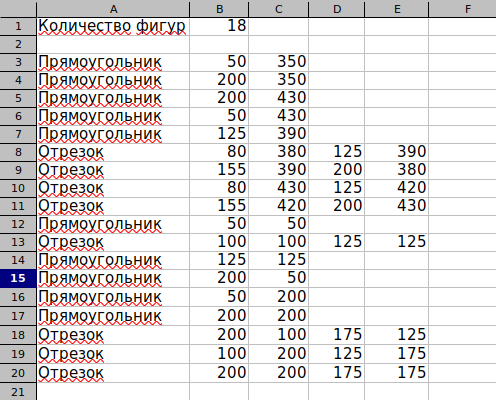
\includegraphics[scale=0.5]{excel5}
	\caption{Получившейся набор данных}
	\label{fig:excel5}
\end{figure}

Таким образом, по данным из презентации нами были сформированы данные excel файла, тем самым нами был рассмотрен процесс экспорта данных в excel файл.